\chapter{Introduction and theory}
\label{chap:theory}

\section{The Standard Model of particle physics}
\subsection{Introduction}

The \SM of particle physics was formulated in the second half of the 20$^{\text{th}}$ century. It has been an immensely successful theory, accurately describing all known processes in high energy physics encountered thus far. The \SM is a gauge theory, in particular a \QFT, in which the universe is made up of interacting fields. The fundamental elements of matter, as well as the fundamental forces which govern their interactions, can be represented as relativistic quantum fields, the excitations of which are manifested as particles. The \SM places the electromagnetic, strong and weak forces into one framework, and unites the electromagnetic and weak forces into the electroweak force. The only force which is not described not the \SM is gravity, since no viable quantum theory of gravity currently exists. This does not affect the predictive power of the \SM however, since the gravitational force is many orders of magnitude weaker than the other three.



%In order to do this, a mechanism ss required to permit the $W^{\pm}$ and $Z$ vector bosons to have mass while allowing the photon to remain masslesss. Such a theory was independently proposed by several theorists~\cite{BroutEnglert,Higgs1,Higgs2,Kibble1,Higgs3,Kibble2}, and is commonly referred to as the Higgs mechanism. In 1964, Higgs postulated that one outcome of this mechanism was that it should yield an observable particle, the Higgs boson~\cite{Higgs2}.

Although the \SM has been very successful as a theory, it falls short of being a “theory of everything", and is clearly incomplete. For instance, it does not accommodate mass terms for neutrinos, which are required to explain the origin of neutrino oscillations observed in many experiments~\cite{SuperK,SNO,DayaBay}. Furthermore, it does not contain a viable candidate for dark matter, which may be needed to explain the mass deficit of the universe~\cite{DM}. Other issues such as the hierarchy problem~\cite{Hierarchy} and the origin of matter-antimatter asymmetry~\cite{Asymmetry} also persist. Clearly, the \SM is incomplete or approximate, and many efforts in modern high energy physics are being made to discover \BSM physics. For examples, detailed studies of the properties of the Higgs boson could provide valuable insight into the nature or indeed existence of \BSM physics.

%Over the decades, the particles which constitute the SM were discovered: the $\tau$ lepton in 1975~\cite{tauDisc}, the $b$ quark in 1977~\cite{bquarkDisc}, the gluon in 1979~\cite{Gluon1,Gluon2,Gluon3}, the $Z$ and $W^{\pm}$ bosons in 1983~\cite{ZDisc,WDisc}, the $t$ quark in 1995~\cite{tquarkDisc1,tquarkDisc2} and the $\nu_{\tau}$ in 2000~\cite{TauNuDisc}. By the turn of the millennium, all but one particle postulated by the SM had been observed: the Higgs boson, which had proved elusive despite decades of searches. The Higgs search prompted the construction of the Large Hadron Collider (LHC) at CERN, and two multi-purpose detectors, ATLAS and CMS, were designed with the Higgs observation as one of their main physics goals. In 2012, the two experiments jointly announced the observation of a Higgs-like particle of mass $\sim$125 GeV, ending a 50-year interval between postulation and discovery~\cite{CMSHDisc,ATLASHDisc}.


\subsection{Particles and Forces}

 The \SM 

\subsection{Electroweak Symmetry Breaking}
\section{The Higgs boson}
According to SM, the Higgs boson's coupling with particles is proportional to their masses. As such, its production modes in the environment of the LHC are dominated by interactions involving the heavier particles of the SM. Typically, the Higgs boson is produced by one of the following mechanisms (Fig. \ref{higgs_prod}, whose cross-sections can be seen in Fig. \ref{H_XS_fig}):

  \begin{figure}[h!]

  \centering
  \subfloat[]{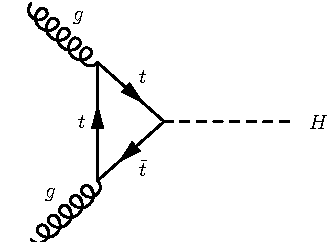
\includegraphics[width=0.3\textwidth]{theoryFigures/ggH.pdf}}
  \subfloat[]{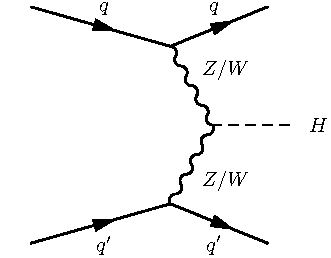
\includegraphics[width=0.3\textwidth]{theoryFigures/vbf.pdf}}\\
  \subfloat[]{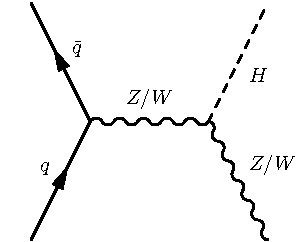
\includegraphics[width=0.3\textwidth]{theoryFigures/wzH.pdf}}
  \subfloat[]{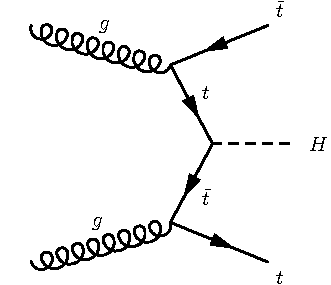
\includegraphics[width=0.3\textwidth]{theoryFigures/ttH.pdf}}
  \caption{Higgs production modes at the LHC: (a) gluon-gluon fusion, via a loop of top quarks, (b) vector boson fusion (VBF), with associated quark production, (c) associated vector boson production and (d) top quark fusion with associated top quark production. }
  \label{fig:theory:higgsproduction}
  \end{figure}

  \newpage
  By the same token, the SM Higgs boson decays to pairs of particles with branching ratios proportional to the square of their mass. The production of a pair of $t$ quarks is not kinematically allowed because their mass is high, so the most likely decay modes are $H \rightarrow ZZ \text{, } W^{\pm}W^{\mp}$, $ b\bar{b}$ and $ \tau^+ \tau^-$. In addition, a small fraction of decays of the Higgs boson ($<1\%$, see Fig. \ref{H_BR_fig}) can occur via a loop diagram to a pair of high-energy photons. The branching fractions and cross sections of these production and decay modes are available in the Handbook of LHC Higgs Cross Sections~\cite{H_XS1,H_XS2}.


  The Higgs boson was discovered in 2012 using data from runs at $\sqrt{s}=7$ and $8$ TeV, and was found to have a mass $m_H \sim 125$ GeV. The signal strengths of the various decay modes at the CMS and ATLAS experiments can be seen in Fig. \ref{sig_strength}. Despite fewer than $1\%$ of Higgs boson decays occurring via $H \rightarrow \gamma \gamma$, this channel played a crucial role in the discovery, and remains one of the two most sensitive methods of studying the Higgs boson. This is in part thanks to the excellent performance of the CMS and ATLAS ECALs, which were able to reach similar sensitivities to the $H\rightarrow \gamma \gamma$ decay mode.

  \subsection{History of Higgs boson searches}
  \subsection{Higgs boson at the LHC}
